\section*{Introducción}

Una ataguía es una estructura temporal utilizada para drenar zonas cubiertas de agua, lo que permite construir en terrenos que, de otra forma, serían inaccesibles \textbf{\cite{madanayaka2018}}. Hay varios factores importantes a considerar al momento de diseñar una ataguía, como el caudal de infiltración, las presiones de poros, la estabilidad de la estructura y, sobre todo, la licuefacción y su factor de seguridad (FS). Este último fenómeno ocurre cuando las presiones de poros alcanzan tal punto que las tensiones internas efectivas entre las partículas del suelo pierden efectividad, y, en consecuencia, la mezcla entre agua y sedimentos actúa como un fluido \textbf{\cite{sumer2009}}.
\\ \\
El presente proyecto tiene como objetivo el estudio y análisis de tres ataguías distintas, donde se busca evaluar sus características mediante cálculos manuales a través de Python, un solver mediante diferencias finitas y un modelo a escala. De esta manera, se busca analizar la efectividad de cada método de análisis, además de hacer una comparación directa entre los resultados obtenidos.
\\ \\
En los cálculos manuales, se utilizó la Ley de Darcy, además de las diferentes ecuaciones necesarias para determinar una red de flujo teórica. De esta forma, se calcularon parámetros como el caudal de infiltración y la presión de poros a lo largo de toda la estructura.
\\ \\
Posteriormente, se desarrolló un solver mediante diferencias finitas, el cual es un método numérico utilizado para calcular diferencias de potenciales en grillas 2D o 3D \textbf{\cite{zhang2005}}. De este modo, al determinar que el flujo va de un potencial mayor a uno menor, se pueden obtener las redes de flujo y, con ello, los distintos parámetros necesarios.
\\ \\
Finalmente, se realizó un modelo a escala, en el que se simuló la ataguía y una falla por licuefacción. Además, se buscó calibrar el modelo computacional en base a los datos obtenidos del modelo real, determinando así cuán efectivo es el cálculo numérico en comparación con la realidad.
\\ \\
El modelo base utilizado a lo largo del informe es el siguiente:

\begin{figure}[H]
    \centering
    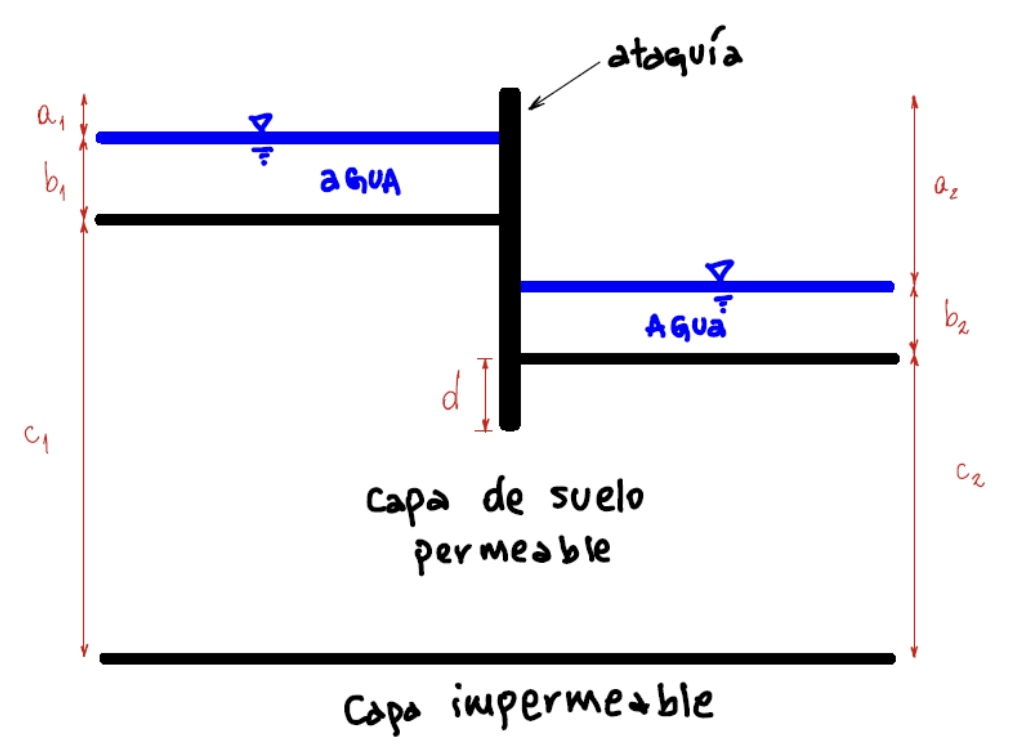
\includegraphics[width=0.45\textwidth]{FOTOS/modelo_base.png}
    \caption{Modelo Base}
    Fuente: Guía de Proyecto
    \label{fig:modelo_base}
\end{figure}

Las medidas para los distintos casos se encuentran en la tabla \textbf{\ref{tab:medidas}}.
